\chapter{Implementation}

    \section{Implementation Specific Constraints}
    
    One of the requirements was that the project should be implemented 
    in the context of the Phalanger project. It should be ready 
    to be plugged in between the Phalanger's front-end and back-end and 
    it should also provide public interface useful for the 
    Phalanger PHP Visual Studio tools.
    
    \paragraph{Abstract Syntax Tree.} Phalanger front-end parses PHP code 
    into an Abstract Syntax Tree (AST) \cite{aho1985compilers} structure. 
    This structure is then traversed by the back-end using the 
    visitor design pattern \cite{gamma1994design}. Phalanger does not 
    use any other intermediate representation than AST and the 
    back end transforms the AST directly to Microsoft Intermediate Language (MSIL).
    
    In order to reduce the memory consumption and provide better 
    modularity, Phalanger code went through minor architecture 
    refactoring before this project was started.     
    The classes representing the AST nodes originally contained 
    the code and data needed for emitting the corresponding 
    MSIL opcodes. This, however, represents 
    a coupling between the front-end and back-end and the 
    front-end could not be used just on its own. In the new 
    version, the classes representing AST nodes are capable 
    of storing additional attributes in an extensible way 
    and the back-end have been rewritten to be an ordinary AST 
    visitor that uses the extensible AST nodes attributes.
    The attributes provide a way to annotate AST nodes 
    with any additional information, which in our case will be 
    the results of the analyses.    
    
    \paragraph{Integrated Development Environment Integration.}
    The PHP Tools for Visual Studio use Phalanger front-end in order to 
    parse PHP code into AST and then the AST is again traversed to provide 
    code completion and other features. All the AST nodes hold necessary 
    pieces of information, for example, the position in the source file or 
    documentation comments.
    
    The aim of this project is to provide the results of type analysis 
    and other analyses to the integrated development environment so 
    that the possible errors and warnings can be visualised.
    
    The longer term aim of this project, not in the scope of this thesis, 
    is to replace the existing algorithms for code completion, 
    ``jump to definition'' and ``find usages'' features. Because 
    with a dynamic language like PHP, it is not trivial to 
    find all the usages of, for example, a class or determine 
    a definition of, for instance, a field accessed on some local variable. 
    In order to provide more precise results, 
    type analysis is needed.
    
    One of the challenging parts of integrated development 
    environment integration is also dealing with incomplete code 
    that is being typed in by the user. Therefore one of the requirements 
    was also that the analysis should be capable of 
    performing an ad-hoc re-analysis of once analysed 
    code with a new statement added. This ad-hoc re-analysis 
    should be, if possible, more effective that doing the 
    whole analysis again.
    
    \section{Overall Design}
    
    The project is divided into several modules.
    \begin{itemize*}
        \item Control Flow Graph,
        \item Intermediate Representation of PHP Code (Phil, RPhil),
        \item Generic Data Flow Analysis Framework, 
        \item Tables with Type and Other Information, 
        \item Concrete Analyses:
        \begin{itemize*}
            \item Dead Code Elimination, 
            \item Aliasing Analysis, 
            \item Constant Propagation,
            \item Type Analysis.
        \end{itemize*}
    \end{itemize*}
    
    The interactions between those modules on a conceptual level 
    when performing an analysis are depicted in diagram \ref{overalldiagram}. 
    Green elements represent extension points. Red arrows represent the 
    core flow of the algorithm.

\begin{figure}[h]  
  \centering
    \includegraphics*[width=\textwidth,height=\textheight,keepaspectratio,viewport=0 55 532 590]{img/ControlFlowModules.pdf}  
    \caption{Control Flow for Phalanger Design Overview\label{overalldiagram}}
\end{figure}    

    \subparagraph*{Intermediate Language.}
    One of the goals of the design was to stay as close as possible 
    to the original AST representation, so that results of an 
    analysis can be easily propagated to an IDE and that the 
    Phalanger back-end does not have to be rewritten in order to 
    leverage the this project.
    
    Control Flow for Phalanger uses two intermediate representations 
    on a conceptual level, however, they are usually not explicitly 
    constructed as described later in the text. The purpose of the 
    intermediate representations is to simplify the design of the 
    analyses.
    
    \emph{Phil} stands for \emph{PHP Intermediate Language} and is very abstract 
    representations close to the original AST. Phil contains 
    only statements and expressions that can be in a Basic Block, 
    therefore it does not contain most of the control flow 
    changing statements like if, switch, or loops. 
    A Phil statement represents the smallest single step 
    of an execution that can change state of variables 
    or global state or throw an exception. Syntactic 
    constructs like \code{\$i++} are unfolded to 
    \code{\$i = \$i + 1}, which is then split to 
    evaluation of binary expression and assignment expression 
    that uses the result of the binary expression. In some sense, 
    Phil can be viewed as a three address code.
    
    \emph{RPhil} stands for \emph{Resolved PHP Intermediate Language}. 
    RPhil is basically a Phil with resolved symbols where possible. 
    By resolved symbols, we mean references to the elements 
    of Type Tables discussed in one of the following paragraphs. 
    In order to resolve the symbols, the module building RPhil 
    can use names explicitly expressed in the code, for example, 
    for direct local variable access \code{\$a}, or results of 
    an analysis, for instance, results of the type analysis to 
    resolve method calls and fields references. 
    RPhil itself is typically consumed by the analyses, 
    so the accuracy of RPhil and subsequently of the 
    analyses results can be improved by iterative execution 
    of the analyses.
    
    \subparagraph*{Analyses.}
    The Data Flow Analysis is performed on Control Flow Graph 
    nodes called basic blocks. Each basic block contains 
    a list of Abstract Syntax Tree elements. This list is 
    then, usually on the fly, transformed to corresponding PHP 
    Intermediate Language elements before they are passed 
    to the flow function of a concrete Data Flow Analysis 
    implementation. 
    
    Basic block can also contain already transformed PHP 
    Intermediate Language elements. However, the interface 
    does not change from the point of view of a concrete 
    Data Flow Analysis implementation.
    
    The Control Flow for Phalanger also contains and allows to 
    plug-in simple analyses that are performed for all 
    basic blocks sequentially without taking the control 
    flow into account. Each basic block is then analysed 
    only once. An example of such analysis is Aliasing Analysis.
    
    The last analysis type, which stands aside, is Dead Code 
    Elimination. It is performed on the Control Flow Graph, 
    but traverses it on its own as opposed to a concrete 
    Data Flow Analysis that only visits basic blocks 
    in order determined by the Data Flow Framework, 
    i.e. does not perform the graph traversal 
    on its own. Control Flow for Phalanger also allows 
    to add custom analyses that are performed on the raw 
    Control Flow Graph.
    
    \subparagraph*{Analyses Results.}
    The results of an analysis can be annotations added 
    to the AST node objects, or annotations of basic blocks, 
    which support extensible attributes in the same way as 
    AST nodes.
    
    The results of an analysis can also be pushed into 
    the Code Tables. Code Tables gather relevant information 
    about code elements like classes, functions, and so on. 
    It is mainly type related information, 
    for example, a return type of a function, 
    but also which parameters are passed by reference or 
    whether the function returns a reference.
    
    \subparagraph*{Type Tables.} This module provides 
    almost the same information about routines, types, 
    global variables and constants as Code Tables. 
    However, in this case the information 
    is abstract, because it might not be directly related 
    to an actual element that can be found in the source code. 
    This is the case of library functions and classes, 
    but it also gives a possibility to merge the information 
    of two or more conditionally declared elements. 
    
    \subparagraph*{Extensibility.}
    The whole project is designed as a class library and 
    framework with many extension points. Some of the 
    functionality can be used independently. For example, 
    Control Flow Graph builder to generate diagrams.
    
    Nonetheless, in order to provide better usability, 
    Control Flow for Phalanger also contains 
    a Facade class \code{AnalysisDriver} 
    that plugs in together all the necessary objects 
    and provides a simple interface to perform a defined 
    analysis of a file or a given piece of code.
    
    \section{The Intermediate Languages and Control Flow Graph}
        The aim of the intermediate languages is to simplify the 
        interface for concrete analyses implementations. 
        However, at the same time, it was desirable to stay as 
        close to the original AST elements as possible in order 
        to easily propagate the results and to easily integrate 
        Control Flow for Phalanger into the Phalanger project.         
        Lastly the intermediate language should stay close enough 
        to PHP code so that PHP specific patterns can be recognized.
        
        \subsection{Phil: PHP Intermediate Language}
        
        \subsubsection*{Motivation}
        The main aim of Phil is to provide a framework for 
        traversing the AST elements in the order of their 
        execution in the smallest execution steps possible 
        with respect to their possible effects to the environment. 
        As opposed to implementing a full blown AST visitor 
        for every analysis, Phil helps to avoid repetitive 
        code that implements the AST structure traversal and 
        breaking down some of the syntactic constructs 
        like \code{\$i++}. As discussed later, a ``Phil element'' 
        is often just a conceptual term, but in reality most 
        of the Phil elements are represented directly by 
        AST elements in order to save resources and stay 
        close to the original AST.
        
        \subsubsection*{Implementation}
        Phil is implemented mainly by two classes \code{PhilVisitor} 
        and \code{Linearizer}, which is a class nested in \code{PhilVisitor}. 
        The \code{PhilVisitor} class implements a variant of the visitor design pattern 
        with virtual \code{Visit*} methods for all the Phil elements. 
        The \code{Linearizer} is implementation of a visitor for the 
        AST elements and it converts them to Phil elements.
        
        An important difference between original AST elements and 
        Phil elements is that Phil does not have a hierarchical structure. 
        Therefore an implementation of the \code{PhilVisitor} class does not 
        need to perform recursive traversal for every visited element.
        
        Under closer look, most of the AST elements correspond 
        to exactly one Phil element\footnote{or they are ignored, 
        which is the case of most control flow changing statements 
        and declaration statements}. 
        Those AST elements are passed to \code{PhilVisitor} as they are. 
        So in this case the \code{Linearizer}, as the name suggests, 
        performs only the traversal and linerizes the AST structure 
        for \code{PhilVisitor} so that it does not have to 
        care about AST structure traversing.
        
        Elements that have to be unfolded into several operations, 
        such as \code{IncDecEx} representing post or pre increment 
        or decrement, have to be represented by more elements. 
        One option would be to create a whole new alternative 
        AST structure that would correspond the unfolded code. 
        In our approach, we reuse the AST element to represent one 
        of the unfolded operations and create new special Phil 
        elements that wrap the original AST element and their 
        only purpose is to indicate the stage of the compound 
        operation. So for example, \code{IncDecEx} is broken down 
        to 
        \begin{itemize*}
            \item \code{Expression} that represents the variable access and 
                is recursively broken down to Phil elements, 
            \item \code{IncDecEx} that represents the binary operation, 
                so the \code{VisitBinaryEx} method is invoked for it on \code{PhilVisitor} as 
                for any other binary operation.
            \item \code{IncDecPhilAssignment} that represents the assignment, 
                and the \code{VisitAssignment} method is invoked for it on \code{PhilVisitor} as 
                for any other assignment.
        \end{itemize*}
        
        Because we have an object instance to represent every Phil element, 
        we do not have to visit them on the fly, they can also be saved into 
        and array and visited by the \code{PhilVisitor} later. This enables 
        us to perform the traversing only once, shall it be a performance issue 
        in the future. It is also possible to crate accurate control flow 
        graphs when it comes to try-catch blocks, because a single AST element, 
        can cause exception in any stage of its evaluation, therefore it should 
        be split into single execution steps and those put into separate 
        basic blocks so that an edge from each of them to the 
        catch block can be created. Note that the design is prepared 
        for this case, but it is not implemented yet.
        
        \subsubsection*{Variables Accesses and Context Information}
        The AST is broken down to small pieces visited by the \code{PhilVisitor}, 
        which does not have to take care about their structure or order. However, 
        sometimes a context information is required in order to handle 
        some elements properly. This is the case of expressions that can be 
        used as left hand side of an assignment or as a parameter passed 
        by reference. In those cases the \code{Visit*} method of \code{PhilVisitor} 
        takes another parameter of type \code{VarUseContext} that identifies the 
        context in which the expression is accessed.
        
        To simplify the AST further, all the accesses to a memory location, be 
        it local variable access, instance field access, or any other, are 
        wrapped in an implementation of abstract class \code{VarLikeConstructInfo}. 
        This class provides unified interface for typical operations performed 
        on this kind of elements. Namely, for example, \code{GetMayReferenceVars}, 
        which returns local variables that this access can point to (typically using 
        the results of points-to analysis).
        
        \subsection{RPhil: Resolved PHP Intermediate Language}
        
        RPhil elements are the same as Phil elements, but with additional 
        information retrieved from Type Tables where possible. 
        \code{RPhilVisitor} implements a variant 
        of the visitor pattern in the same way as \code{PhilVisitor}, but 
        the virtual \code{Visit*} methods take additional parameters 
        that provide this kind of information.
        
        A simple example is direct static field access, in which 
        case the resolving is trivial, because the \code{RPhilVisitor} 
        can get the class and field's name directly from the AST element. 
        However, even a direct object's method access, is challenging, 
        because we do not know the type of the expression that is 
        being dereferenced using \code{->} operator.
        
        RPhil does not perform any analysis in order to resolve such 
        cases, but by convention it looks for certain additional 
        attributes attached to the AST elements in question. Those 
        attributes are expected to be filled in by analyses. Concretely, 
        every expression can be annotated with its type and value.
    
        \subsection{Control Flow Graph}
        
        Control Flow Graphs are constructed by an implementation of the 
        AST visitor. The class holds an instance of a basic block that 
        is being currently constructed. Statements are sequentially visited, 
        and those that do not change the flow of the control are just added 
        to the current basic block. Statements that change the flow lead to 
        a creation of new basic blocks that have incoming edges from the 
        previous basic block.
        
        This structure works for well structured code, but PHP permits 
        \code{goto} statements, especially forward ones are problematic, 
        because at the moment the \code{goto} statement is being processed, 
        the basic block for the target might not be constructed yet. 
        For this purpose a table of \code{goto} statements and all the labels 
        is created during the control flow graph construction and the 
        \code{goto} statements are connected to their \code{labels} at the 
        end once the whole routine body is processed.
        
        \subsubsection*{Exceptions}
        When a try code block is processed, every statement is placed in 
        its own basic block that is connected to the basic block of the 
        consecutive statement and connected to all the possible catch code blocks.
        
        The possible catch blocks are chosen pessimistically, so 
        a statement in try code block is connected to all the catch code blocks, 
        even nested ones, up to a catch block that catches generic \code{Exception} 
        or to the graph's \emph{exit} basic block.
        
        \subsubsection*{Edges}
        Control Flow Graph edges can have an optional attribute which 
        states the expression that has to hold if this edge is taken 
        during the execution. For example, an edge to then branch of 
        \code{if (\$x==3)} will have expression \code{\$x==3} and the 
        analyses may work out from it that \code{\$x} is equal to 
        \code{3} in the basic block corresponding to the then branch.
        
    \section{Data Flow Analysis}
        A data flow analysis (DFA) in general can be performed on any graph, 
        the implementation of Control 
        and so even in our case, we did not want it to be tied 
        Flow Graph. For this purpose, our implementation of DFA is 
        performed on interfaces that Control Flow Graph implements, 
        but they can be implemented, for example, by definition-use 
        graph\cite{aho1985compilers} and DFA can be run on this graph too.
        The interfaces are depicted in figure \ref{graphifaces}.
        
\begin{figure}[h]  
  \centering
    \includegraphics*[width=\textwidth,height=\textheight,keepaspectratio]{img/graph-ifaces.png}  
    \caption{Generic Graph Interfaces for DFA\label{graphifaces}}
\end{figure}    

        The generic data flow framework handles the order in which the 
        graph nodes should be visited, compares the input and output 
        data flows and decides when the analysis has reached a fix-point. 
        However the concrete type of data flow, operations with data 
        flow instances and the transfer function are left to be defined 
        by a concrete analysis. In Control Flow for 
        Phalanger, two types of analysis can implemented. The basic one 
        processes only nodes; the ``branching'' one also processes edges, 
        in which case it can take the branching expressions of Control 
        Flow Graph into account, for example, but in general any information 
        that the concrete implementation of \code{IEdge} can provide.
        
        The operations with data flow objects could be carried out by the 
        objects themselves, but this would mean that already existing 
        classes that happens to be suitable for being a data flow would 
        have to be wrapped. And also one data flow representation, could 
        not have different operations for different analyses. An example 
        of this is \code{BitVector} class from .NET class library: it 
        cannot implement any additional interface, and some analysis 
        perform union of two vectors as the meet operation, while 
        others perform intersection.
        
        Nonetheless, having the data flow objects implement the operations by 
        themselves is more convenient and allows better encapsulation. 
        Because Control Flow for Phalanger is meant as a framework for as 
        well as software on its own, both scenarios are supported and 
        some convenient generics based implementations of required 
        interfaces are provided. The whole design is captured in 
        diagram \ref{dataflowifaces}.
        
\begin{figure}[h]  
  \centering
    \includegraphics*[width=\textwidth,height=\textheight,keepaspectratio]{img/dataflow-ifaces.png}  
    \caption{Interfaces for concrete Data Flow Analyses\label{dataflowifaces}}
\end{figure}

        A simple example of concrete Data Flow Analysis is the built-in 
        constant propagation analysis, which is discussed in one of the 
        following sections.
        
    \section{Tables}
        Tables module responsibility is to maintain a database 
        of symbols that can be referenced from the code. 
        This module distinguishes between two kinds of symbols: 
        symbols that can be found in the analysed code, and external 
        symbols, which could be library functions, for example.
        
        \subsection{Type Tables}
        
        The most generic interface \code{ITypeTables} for querying 
        the tables database merges the two kinds of symbols 
        and provides mainly abstract type related information. 
        The structure is shown in class diagram \ref{tablesifaces}.
        
\begin{figure}[h]  
  \centering
    \includegraphics*[width=\textwidth,height=\textheight,keepaspectratio]{img/tables-ifaces.png}  
    \caption{The Interface of Type Tables\label{tablesifaces}}
\end{figure}

        The tables need to know a context from which the 
        query is made, because certain names can refer 
        to different symbols in different namespaces 
        for example. The \code{ContextManager} class maintains 
        the current context and the consumers of the \code{ITypeTables} 
        should invoke \code{EnterContext} and \code{LeaveContext} on its 
        \code{ContextManager} to provide the correct context 
        for their queries.

        Global variables and fields provide two pieces type 
        information: \code{ExpectedType} is checked when a 
        value is assigned to that variable and the \code{Type} 
        is used as the type of an expression that accesses 
        the variable. Typically, the expected type is what 
        the PHPDoc states and the ``type'' can be either what 
        PHPDoc states or type inferred from all the assignments 
        made to that variable.
        
        The fact that results of \code{ITypeTables} queries 
        are only abstract type information not related to a 
        concrete element in code, allows us to support built-in 
        functions and classes and also to handle conditional 
        declarations by merging the type information from 
        all the occurrences found. However, this has not 
        been implemented, but the design is prepared for it, 
        shall it be considered an important feature in the future. 
        At the moment, if two or more declarations are found, 
        the Type Tables behave as if they did not know the 
        element at all, which preserves correctness for the 
        price of loosing precision.
        
        The basic implementation of \code{ITypeTables} is 
        \code{Tables} class, which follows a variant of the 
        composite design pattern. It gets a list of other 
        \code{ITypeTables} implementations as its constructor 
        parameter and queries those one by one until the 
        symbol is found, or returns a value that indicates 
        that the symbol was not found. The actual implementations 
        of \code{ITypeTables} include Code Tables discussed 
        later and can include user defined \code{ITypeTables} 
        implementation that provides information about 
        built-in functions and classes.
    
        \subsection{Code Tables}
        Code Tables provide information related to concrete elements in 
        the analysed code. So in this case not abstract type related 
        information is provided, but a reference to the AST element 
        with the declaration. Another difference to Type Tables is that 
        Code Tables can return more results for one symbol name, 
        which is because of conditional declarations. 
        Other than that, the interface is similar to the one of 
        Type Tables.
        
        \subsection{Dependency Resolver}
        Dependency Resolver serves as an adapter of Code Tables interface 
        to the Type Tables interface. However, in the case of routines, 
        the routine's declaration AST element does not provide all the 
        necessary type information straight away. Especially inferred 
        return type, which is results of Type Analysis, will not be 
        available if the analysis has not been performed yet.
        
        By convention, all the necessary information for analysing a 
        routine and the results of the type analysis are stored in an 
        instance of \code{RoutineContext} class in the additional attributes 
        of the routine's declaration AST element. Since this AST element 
        is returned by Code Tables, Dependency Resolver can check if 
        the element has the annotation and if so return it as the result, 
        and if not, it can start analysis of the routine. However, 
        there can be cyclic references between routines, so Dependency 
        Resolver also maintains a list of all the routines that are 
        currently being analysed and if a routine is already in the list, 
        default type information is returned as the query result instead 
        of performing the analysis.
        
        \subsection{RoutineContext}
        
        \code{RoutineContext} class provides information about a routine 
        needed for most of the analysis in order to analyse the routine. 
        All the local variables, parameters and referenced global and 
        static variables are numbered and accessed through their number 
        instead of their name. The data \code{RoutineContext} provides are:
        
        \begin{itemize*}
            \item Lists of
                \begin{itemize*}
                    \item all referenced types in the routine's body,
                    \item all referenced variables (local, global, static).
                \end{itemize*}
            \item Results of the points-to analysis: lists of all variables that
                \begin{itemize*}
                    \item given variable can point to, 
                    \item can be pointed to by another variable, 
                    \item are captured by reference by some lambda function.
                \end{itemize*}
            \item Control Flow Graph.
            \item Signature information -- implementation of \code{IRoutineTypesInfo} from Type Tables.
            \item Results of Type Analysis:
                \begin{itemize*}
                    \item inferred return type.
                \end{itemize*}
        \end{itemize*}
        
    
    \section{Analyses}
        \subsection{Dead Code Elimination}
        
        The Dead Code Elimination is based on the Reverse Post Order 
        algorithm, which is supposed to order nodes in a way that 
        is the most beneficial for Data Flow Analysis and has to be 
        done anyway in order to perform Data Flow Analysis.
        
        Note that the Reverse Post Order algorithm as a part 
        of the Data Flow Analysis module is implemented 
        in a generic way for any \code{IGraph} implementations. 
        
        The algorithm performs a graph search from the \emph{Start} 
        node and after it finishes, the unvisited nodes are 
        at the end of the list with all the nodes. At this point, 
        the list with all the nodes is traversed from the last 
        element and the unvisited nodes are removed until a 
        first visited node is reached.
        
        The Control Flow Graph is design allows to mark 
        some edges as ``not executable'' if the branching 
        condition is always false. Such edges will be ignored 
        when the Dead Code Elimination is performed, however, 
        the tagging of edges with false branching condition 
        has not been implemented in the final version.        
        
        \subsection{Constant Propagation}
        Constant Propagation represents a simple example of non-branched 
        implementation of a concrete Data Flow Analysis. 
        
        The lattice for the data flow values of single variable is 
        depicted in figure \ref{constlattice}. The Data Flow type is class 
        \code{ConstantPropagationDataFlow}, which wraps an array 
        that contains the value of each variable. Note 
        that the variables names are already converted to numbers by 
        \code{RoutineContext} and those numbers serve as indexes into this array.
        The value is an \code{object} instance, so it can be \code{null}, which 
        is the least element of the lattice, or its value can be concrete 
        singleton object instance that by convention represents 
        \code{NotAConstant}, which is the greatest element of the lattice.
        
\begin{figure}[h]  
  \centering
    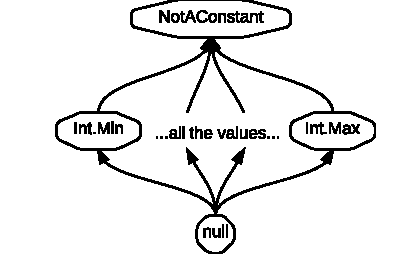
\includegraphics{img/ConstLattice.pdf}  
    \caption{The Lattice for Constant Propagation\label{constlattice}}
\end{figure}        
        
        The transfer function annotates every expression 
        with its constant value if possible. An access to a 
        variable is annotated with this variable's value 
        from the data flow, some expressions can be symbolically 
        executed using the annotations to get operands values, 
        and constants are annotated with their value retrieved 
        from Type Tables.
        
        The data flow is updated only for assignment statement, 
        reference assignment statement and for function call, 
        because some local variables can be passed by reference, 
        which can change their value. The right hand side of 
        the assignment is an expression, which should already by 
        annotated with its value that is used for the data 
        flow value.
        

        

    \section{Type Analysis}
        \note{
        \begin{itemize}
            \item Type Information representation
            \item Data Flow representation
            \item AST annotations
        \end{itemize}}

    \section{The Analyser pipeline and AnalysisDriver}
        \note{Description of the high level public interface 
        and the phases of the full analysis process.}
